\section{Methodology for Causal Inference}
\label{sec:causal-methodology}
\subsection{Causal Diagram and Variable Definitions}

We model the relationships between article content, sentiment, and ideology using the causal diagram in Figure~\ref{fig:causal_diagram}, which formalizes our assumptions about the data-generating process and determines which variables must be controlled for to obtain unbiased causal estimates.

We define the following variables:
\begin{itemize}
    \item $X$: (text) the full article text parsed from the publishing source.
    \item $T$: (topic tags) AllSides-assigned topic tags (e.g.\ Politics, Government Efficiency, Foreign Affairs).
    \item $F$: (sentiment) sentiment toward each topic, inferred from article text using an LLM.
    \item $Y$: (ideology) the political ideology label assigned by AllSides.
\end{itemize}

\begin{figure}[h]
    \centering
    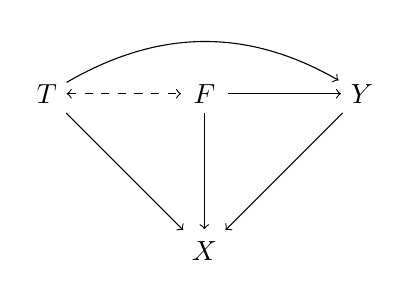
\begin{tikzpicture}[->,shorten >=1pt,auto,node distance=2cm]
      \tikzstyle{every state}=[]

      \node(text) {$X$};
      \node(sentiment) [above of=text] {$F$} edge [->] (text);
      \node(ideology) [right of=sentiment] {$Y$} edge [<-] (sentiment) edge [->] (text);
      \node(topic) [left of=sentiment] {$T$} edge [->] (text) edge [->, bend left] (ideology) edge [<->, dashed] (sentiment);
    \end{tikzpicture}
    \caption{Causal diagram for article ideology classification.}
    \label{fig:causal_diagram}
\end{figure}

Each arrow represents a hypothesized causal direction. The arrow from $Y$ to $X$ reflects that ideology shapes article content and framing. The arrow from $F$ to $X$ reflects that sentiment toward a topic influences how that topic is discussed. The bidirectional dashed arrow between $T$ and $F$ captures the mutual relationship between topics and sentiment: certain topics tend to evoke particular sentiments, while prevailing sentiment patterns influence which topics receive coverage.

In practice, each node expands into many variables. Figure~\ref{fig:causal3} illustrates this: each sentiment node $F$ corresponds to a distinct topic, and sentiment toward one topic ($F_T$, the treatment) may influence sentiment toward other topics ($F_{M_1}, F_{M_2}, \ldots$, the mediators), which in turn affect ideology classification $Y$. The structural relationships \textit{between} variable types remain as in Figure~\ref{fig:causal_diagram}; what changes is the dimensionality \textit{within} each node.

\begin{figure}[h!]
  \centering
  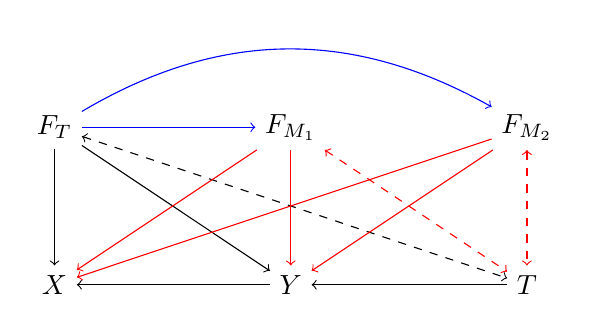
\begin{tikzpicture}[->,auto]
    % Top row: the three F's
    \node (FT)   at (0,0)   {$F_{T}$};
    \node (FM1)  at (3,0)   {$F_{M_1}$};
    \node (FM2)  at (6,0)   {$F_{M_2}$};

    % Bottom row: the three observed variables
    \node (Xabs) at (0,-2)  {$X$};
    \node (Y)    at (3,-2)  {$Y$};
    \node (T)    at (6,-2)  {$T$};

    % Edges from F_T
    \draw[->]           (FT) -- (Y);
    \draw[->]  (FT) -- (Xabs);
    \draw[<->, dashed]  (FT) -- (T);

    % Edges from X_abs and T to Y
    \draw[<-]           (Xabs) -- (Y);
    \draw[->]  (T) to (Y);

    % Edges for F_{M_1}
    \draw[->, red]             (FM1) -- (Y);
    \draw[->, red]    (FM1) -- (Xabs);
    \draw[<->, dashed, red]    (FM1) -- (T);
    \draw[<-, blue]            (FM1) -- (FT);

    % Edges for F_{M_2}
    \draw[->, red]             (FM2) -- (Y);
    \draw[->, red]    (FM2) -- (Xabs);
    \draw[<->, dashed, red]    (FM2) -- (T);
    \draw[<-, blue, bend right] (FM2) to (FT);
  \end{tikzpicture}
  \caption{Experimental setup: sentiment variables as mediators. Blue arrows show treatment-to-mediator paths; red shows mediator-to-outcome paths.}
  \label{fig:causal3}
\end{figure}

The roles of each variable in the estimation framework are:

\paragraph{Treatment Variable ($F_T$):} Sentiment toward a specific topic of interest (e.g., sentiment toward ``Immigration'' or ``Healthcare''). This is the variable whose causal effect on ideology we seek to estimate.

\paragraph{Outcome Variable ($Y$):} The ideology label (Left/Center/Right) assigned to the article.

\paragraph{Mediator Variables ($F_{M_1}, F_{M_2}, \ldots$):} Sentiment toward all other topics present in the article. These lie on the causal pathway between treatment sentiment and ideology: sentiment toward one topic may influence sentiment toward related topics, which in turn affects ideology classification. Blue arrows in Figure~\ref{fig:causal3} show these paths.

\paragraph{Confounder Variables:} $T$ (topic presence) is the primary confounder, since the presence of a topic influences both sentiment toward it and the overall ideological character of the article. $X$ (text content) acts as a collider, influenced by both sentiment and ideology.

We restrict the analysis to articles containing the treatment topic, preventing invalid comparisons between articles that discuss a topic and those that do not. This design supports estimation of Average Treatment Effects (ATE), Conditional Average Treatment Effects (CATE), Natural Direct Effects (NDE), and Natural Indirect Effects (NIE).

\subsection{Data Collection}
We use the AllSides extended dataset described in Section~\ref{sec:dataset}. To extract sentiment variables ($F$), we apply a two-step process to the full article text ($X$):

\begin{enumerate}
\item \textbf{Entity and Sentiment Analysis:} Named entities and key concepts are extracted from the corpus. The \texttt{llama-3.3-70b-versatile} model assigns sentiment polarity to each entity on a continuous scale from $-1.0$ (strongly negative) to $+1.0$ (strongly positive). This model was chosen for its sensitivity to contextual nuances compared to smaller alternatives.

\item \textbf{Entity-to-Topic Association:} The \texttt{llama3-70b-8192} model quantifies how strongly each extracted entity relates to predefined AllSides topic tags. The model avoids spurious correlations---for example, correctly distinguishing between terrorism as a broad concept and specific incidents like the 2019 Christchurch shooting when assigning the entity ``shooting'' to a topic. Entity sentiment scores are then aggregated by topic tag to produce a per-topic sentiment profile for each article.
\end{enumerate}

\subsection{Experimental Design}
\label{sec:experimental-design}

We perform all analyses on the test set of the AllSides dataset to ensure fair comparison across annotation sources. To identify the topical structure of this set, we apply the Louvain community detection algorithm to a co-occurrence graph of topic tags, where nodes are tags and edge weights reflect how often two tags appear together in the same article. Self-loops allow single-tag articles to form their own communities. This yields a modularity score of 0.498 across 12 communities, with community sizes ranging from 1 to 199 tags.

\begin{table}[h]
    \centering
    \begin{tabular}{lcc}
    \toprule
    \textbf{Topic Tag} & \textbf{Articles} & \textbf{Community} \\
    \midrule
    politics & 756 & 2 \\
    donald\_trump & 712 & 11 \\
    world & 503 & 4 \\
    elections & 451 & 11 \\
    white\_house & 444 & 2 \\
    \bottomrule
    \end{tabular}
    \caption{Top five topic tags by frequency in the test set.}
    \label{tab:top-tags}
\end{table}

We focus on the five most frequent topic tags (Table~\ref{tab:top-tags}), which provide sufficient statistical power while spanning three distinct communities (Figure~\ref{fig:louvain}): political figures and electoral processes (Community 11: \textit{donald\_trump}, \textit{elections}), institutional politics (Community 2: \textit{politics}, \textit{white\_house}), and international affairs (Community 4: \textit{world}).

\begin{figure}[h!]
    \centering
    \includegraphics[width=0.7\textwidth]{sections/images/louvain_communities.png}
    \caption{Louvain community detection on the topic tag co-occurrence graph for the top five tags.}
    \label{fig:louvain}
\end{figure}

Our primary experiment examines the bidirectional relationship between sentiment toward \textit{donald\_trump} and sentiment toward \textit{politics} in shaping ideology classification. We test two competing hypotheses: (1) Trump sentiment drives general political sentiment, which then shapes ideology; versus (2) broader political sentiment shapes Trump-specific framing, with Trump sentiment mediating the path to ideology. We use NIE/NDE decomposition and bidirectional mediation to determine the dominant pathway.

Building on this, we test whether the mediation pattern generalizes: do institutional political topics (Community 2) systematically mediate the effects of political figure sentiment (Community 11) on ideology? We estimate CATEs for different combinations of these sentiment variables, testing whether the Trump--politics dynamic reflects a broader structural relationship between individual figures and institutional framing.

All experiments are conducted across three annotation paradigms:

\begin{enumerate}
    \item \textbf{Human annotations:} Manual ideology labels from AllSides, serving as ground truth.

    \item \textbf{Fine-tuned RoBERTa:} Predictions from the best-performing fine-tuned classifier from Section~\ref{sec:continued-pretraining}.

    \item \textbf{Fine-tuned GPT-4o-mini:} Predictions from the fine-tuned GPT model from Section~\ref{sec:llm-finetuning}.
\end{enumerate}

This three-way comparison allows us to examine whether causal relationships are stable across annotation approaches or vary systematically between human judgment, traditional classifiers, and large language models.

\subsubsection{Double Machine Learning}
\label{sec:dml}

Ordinary regression of $Y$ on $F_T$ is biased when confounders $W$ predict both $F_T$ and $Y$. For example, articles from right-leaning outlets may mention the FBI more often \emph{and} receive right-leaning labels, creating a spurious positive correlation between FBI sentiment and ideology that is driven by outlet identity rather than sentiment itself.

DML~\cite{chernozhukov2018} removes this bias through two-stage residualization:
\begin{enumerate}
  \item Fit $\hat{g}(W)$ to predict $Y$ from $W$ alone; compute residuals $\tilde{Y} = Y - \hat{g}(W)$.
  \item Fit $\hat{m}(W)$ to predict $F_T$ from $W$ alone; compute residuals $\tilde{F}_T = F_T - \hat{m}(W)$.
  \item Regress $\tilde{Y}$ on $\tilde{F}_T$ to obtain the ATE.
\end{enumerate}

After residualization, both $Y$ and $F_T$ have had their confounder-explained variation removed, so the final regression captures only the direct sentiment--ideology relationship that topic presence cannot explain. We use \texttt{LinearDML} from EconML~\citep{econml} with Random Forest base learners (\num{200} trees, maximum depth~5) and $k = 5$-fold cross-fitting.

The ATE is interpreted as: ``holding topic-presence composition constant, a one-unit increase in $F_T$ shifts the expected ideology label by $\widehat{\text{ATE}}$ units on the $[0,2]$ scale.''

\subsubsection{Mediation Analysis}
\label{sec:mediation-design}

The Total Effect (TE) decomposes into:

\begin{equation}
  \underbrace{\text{TE}}_{\text{Total}} =
  \underbrace{\text{NDE}}_{\substack{\text{Natural Direct}\\ \text{Effect}}} +
  \underbrace{\text{NIE}}_{\substack{\text{Natural Indirect}\\ \text{Effect}}}
\end{equation}

\begin{itemize}
  \item The \textbf{NDE} is the portion of the treatment effect that acts directly on the outcome, bypassing the mediator.
  \item The \textbf{NIE} acts through the mediator: $F_T \to F_M \to Y$.
\end{itemize}

For example, positive Trump sentiment ($F_T$) may incline an article toward positive Politics framing ($F_M$). If positive Politics sentiment then influences the ideology classifier, the NIE captures that indirect path; the NDE captures all remaining direct pathways.

We estimate NDE and NIE using nested DML estimators with $B = \num{2000}$ bootstrap iterations for 95\% confidence intervals. Because the TE confidence interval consistently includes zero in our results (see Section~\ref{sec:mediation-results}), we suppress the proportional mediation $(\text{NIE}/\text{TE})$ to avoid division-by-near-zero artifacts.

\subsubsection{Treatment Encoding and Contrasts}
\label{sec:treatment-encoding}

Two treatment encodings are used:

\begin{description}
  \item[Continuous] The raw sentiment score on the $[-100, +100]$ scale, standardized (zero mean, unit variance) before estimation, so that the ATE represents the effect of a one-standard-deviation increase. This preserves fine-grained variation: a score of $+45$ carries more positive framing than $+1$.
  \item[Discrete] The raw score sign-encoded into $\{-1, 0, +1\}$ (Negative, Neutral, Positive) using thresholds at $-\epsilon$ and $+\epsilon$. The ATE represents the effect of moving one sentiment level (e.g., Negative to Neutral).
\end{description}

For the mediation analysis, treatment contrasts are evaluated at the interquartile range ($Q25 \to Q75$, primary) and the 10th--90th percentile range ($P10 \to P90$, secondary), computed from the empirical distribution of the continuous treatment score in the filtered subsample. For example, a CATE of $-0.21$ for Left-leaning outlets means that increasing Trump sentiment from $Q25$ to $Q75$ is associated with a $-0.21$ shift in ideology on the $[0,2]$ scale.

\subsubsection{Confounder Dimensionality Reduction}
\label{sec:pca}

The topic-presence indicator matrix $W$ has \num{625} columns---one per AllSides topic tag. We apply PCA to $W$, retaining components that together explain 95\% of the variance (capped at 50 components). This reduces $W$ to between 20 and 45 components depending on the filtered subsample, improving numerical stability without discarding meaningful between-topic variation.

Missing topic-presence values are imputed as 0, reflecting the semantic equivalence of ``topic absent'' and ``indicator = 0.'' Sentiment scores for absent topics are similarly imputed as 0 (neutral).

\subsubsection{Multi-Treatment DML}
\label{sec:multi-treatment-design}

While mediation analysis fits one model per topic pair $(F_T, F_M)$, a complementary approach fits a \emph{single} model with all qualifying topic sentiments simultaneously as a treatment matrix $\mathbf{T} \in \mathbb{R}^{N \times k}$. This controls for correlations among sentiments and yields one ATE per topic, interpreted as the effect of that topic's sentiment \emph{holding all other topic sentiments constant}.

Topics are included only if they appear in at least 50 articles ($N_\text{topic} \geq 50$). Of the 625 topic columns, 11 meet this threshold: \textbf{Donald Trump}, \textbf{Politics}, \textbf{Media Bias}, \textbf{Race and Racism}, \textbf{FBI}, \textbf{Defense and Security}, \textbf{Hillary Clinton}, \textbf{LGBTQ Issues}, \textbf{Russia Probe}, \textbf{Media Watch}, and \textbf{Economy and Jobs}. Both continuous and discrete encodings are run for each dataset.

\subsection{Mediation Analysis Results}
\label{sec:mediation-results}

Two treatment--mediator configurations are evaluated: \textbf{Donald Trump sentiment as treatment} with Politics sentiment as mediator ($N = 233$ articles), and \textbf{Politics sentiment as treatment} with Donald Trump sentiment as mediator ($N = 594$ articles). The smaller $N$ in the Trump condition reflects the sparsity of Trump-tagged articles in the corpus.

% ..............................................................................
\subsubsection{Donald Trump Sentiment as Treatment}
\label{sec:mediation-trump}
% ..............................................................................

Table~\ref{tab:te-trump} reports Total Effect estimates for both percentile contrasts across the three annotation paradigms. The treatment window is identical across all three datasets ($Q25 = -0.7$, $Q75 = +0.1$; $P10 = -1.1$, $P90 = +0.3$), so differences across paradigms arise entirely from differences in ideology labels $Y$.

\begin{table}[ht]
  \centering
  \caption{Total Effect (TE) of Donald Trump sentiment on ideology label for
    two percentile contrasts. $N = 233$ articles. No estimate is statistically
    significant ($p < 0.05$); all 95\% CIs include zero.}
  \label{tab:te-trump}
  \sisetup{table-format=+1.3}
  \begin{tabular}{llS[table-format=+1.3]S[table-format=+1.3]S[table-format=+1.3]S[table-format=+1.3]S[table-format=+1.3]}
    \toprule
    \textbf{Paradigm} & \textbf{Contrast} &
      {\textbf{TE}} &
      {\textbf{CI lower}} & {\textbf{CI upper}} &
      {\textbf{NDE}} & {\textbf{NIE}} \\
    \midrule
    Human
      & $Q25 \to Q75$  & -0.254 & -0.934 & +0.426 & -0.160 & -0.094 \\
    Human
      & $P10 \to P90$  & -0.438 & -1.612 & +0.735 & -0.263 & -0.175 \\
    \addlinespace
    Fine-tuned RoBERTa
      & $Q25 \to Q75$  & -0.122 & -0.825 & +0.581 & -0.043 & -0.079 \\
    Fine-tuned RoBERTa
      & $P10 \to P90$  & -0.211 & -1.424 & +1.002 & -0.098 & -0.112 \\
    \addlinespace
    GPT-4o-mini
      & $Q25 \to Q75$  & +0.087 & -0.522 & +0.695 & +0.043 & +0.044 \\
    GPT-4o-mini
      & $P10 \to P90$  & +0.150 & -0.900 & +1.199 & +0.122 & +0.027 \\
    \bottomrule
  \end{tabular}
\end{table}

The most striking finding is a \textbf{sign reversal} in the Total Effect: Human and Fine-tuned RoBERTa estimates are negative (more positive Trump sentiment $\to$ ideology shifts toward Left), while GPT-4o-mini estimates are positive (more positive Trump sentiment $\to$ ideology shifts toward Right). Since the treatment window and article set are identical, this reversal reflects entirely how each labelling system classifies the same 233 articles. No estimate reaches statistical significance; all 95\% confidence intervals span zero.

The NDE accounts for the majority of the TE in all runs ($|\text{NDE}| > |\text{NIE}|$ in every case), indicating that most of the estimated effect does not route through the Politics sentiment mediator.

% TODO: validate images before restoring this figure
%\begin{figure}[ht]
%  \centering
%  \begin{subfigure}[t]{0.32\textwidth}
%    \includegraphics[width=\textwidth]{sections/images/allsides_df_test/bin_pca_t_Donald_Trump_m_Politics_2000/mediation_forest_plot.png}
%    \caption{Human annotations}
%  \end{subfigure}
%  \hfill
%  \begin{subfigure}[t]{0.32\textwidth}
%    \includegraphics[width=\textwidth]{sections/images/best_model_allsides_df_test/bin_pca_t_Donald_Trump_m_Politics_2000/mediation_forest_plot.png}
%    \caption{Fine-tuned RoBERTa}
%  \end{subfigure}
%  \hfill
%  \begin{subfigure}[t]{0.32\textwidth}
%    \includegraphics[width=\textwidth]{sections/images/gpt_finetuned_allsides_test/bin_pca_t_Donald_Trump_m_Politics_2000/mediation_forest_plot.png}
%    \caption{GPT-4o-mini}
%  \end{subfigure}
%  \caption{NDE and NIE estimates for Donald Trump sentiment treatment
%    across the three annotation paradigms ($Q25 \to Q75$ contrast).
%    Error bars show 95\% bootstrap confidence intervals.  All intervals
%    include zero; the NDE sign reverses between GPT-4o-mini and the other two
%    paradigms.}
%  \label{fig:mediation-trump}
%\end{figure}

% ..............................................................................
\subsubsection{Politics Sentiment as Treatment}
\label{sec:mediation-politics}
% ..............................................................................

Table~\ref{tab:te-politics} reports the mirrored configuration: Politics sentiment as treatment ($Q25 = -0.3$, $Q75 = 0.0$; $P10 = -0.8$, $P90 = +0.3$) with Donald Trump sentiment as mediator ($N = 594$ articles).

\begin{table}[ht]
  \centering
  \caption{Total Effect (TE) of Politics sentiment on ideology label.
    $N = 594$ articles. All estimates are non-significant; directions are
    consistent across paradigms.}
  \label{tab:te-politics}
  \sisetup{table-format=+1.3}
  \begin{tabular}{llS[table-format=+1.3]S[table-format=+1.3]S[table-format=+1.3]S[table-format=+1.3]S[table-format=+1.3]}
    \toprule
    \textbf{Paradigm} & \textbf{Contrast} &
      {\textbf{TE}} &
      {\textbf{CI lower}} & {\textbf{CI upper}} &
      {\textbf{NDE}} & {\textbf{NIE}} \\
    \midrule
    Human
      & $Q25 \to Q75$  & +0.027 & -0.241 & +0.296 & +0.030 & -0.003 \\
    Human
      & $P10 \to P90$  & +0.097 & -0.860 & +1.054 & +0.099 & -0.002 \\
    \addlinespace
    Fine-tuned RoBERTa
      & $Q25 \to Q75$  & +0.047 & -0.198 & +0.292 & +0.041 & +0.007 \\
    Fine-tuned RoBERTa
      & $P10 \to P90$  & +0.169 & -0.705 & +1.043 & +0.140 & +0.029 \\
    \addlinespace
    GPT-4o-mini
      & $Q25 \to Q75$  & +0.039 & -0.193 & +0.271 & +0.014 & +0.025 \\
    GPT-4o-mini
      & $P10 \to P90$  & +0.140 & -0.687 & +0.968 & +0.048 & +0.093 \\
    \bottomrule
  \end{tabular}
\end{table}

In contrast to the Trump treatment, the Politics treatment yields \textbf{consistent positive directions} across all three paradigms, though no estimate reaches statistical significance. The NIE is near zero for Human labels ($-0.003$ and $-0.002$), slightly larger for Fine-tuned RoBERTa ($+0.007$ and $+0.029$), and largest for GPT-4o-mini ($+0.025$ and $+0.093$). This gradient suggests GPT-4o-mini labels capture a stronger coupling between Politics and Trump sentiments, creating a more pronounced indirect pathway.

% TODO: validate images before restoring this figure
%\begin{figure}[ht]
%  \centering
%  \begin{subfigure}[t]{0.32\textwidth}
%    \includegraphics[width=\textwidth]{sections/images/allsides_df_test/bin_pca_t_Politics_m_Donald_Trump_2000/mediation_forest_plot.png}
%    \caption{Human annotations}
%  \end{subfigure}
%  \hfill
%  \begin{subfigure}[t]{0.32\textwidth}
%    \includegraphics[width=\textwidth]{sections/images/best_model_allsides_df_test/bin_pca_t_Politics_m_Donald_Trump_2000/mediation_forest_plot.png}
%    \caption{Fine-tuned RoBERTa}
%  \end{subfigure}
%  \hfill
%  \begin{subfigure}[t]{0.32\textwidth}
%    \includegraphics[width=\textwidth]{sections/images/gpt_finetuned_allsides_test/bin_pca_t_Politics_m_Donald_Trump_2000/mediation_forest_plot.png}
%    \caption{GPT-4o-mini}
%  \end{subfigure}
%  \caption{NDE and NIE estimates for Politics sentiment treatment
%    across the three annotation paradigms.  All estimates are positive
%    and directionally consistent, but no confidence interval excludes zero.}
%  \label{fig:mediation-politics}
%\end{figure}

% ..............................................................................
\subsubsection{Conditional Average Treatment Effects by Outlet Ideology}
\label{sec:cate-results}
% ..............................................................................

To test whether the sentiment--ideology relationship differs by outlet type, we estimate CATEs using a Causal Forest DML~\citep{wager2018forests} and group results by outlet ideology (Left, Centre, Right). Heterogeneity here would indicate that the effect of sentiment on classification is moderated by the outlet's baseline ideology.

Tables~\ref{tab:cate-trump} and~\ref{tab:cate-politics} report mean CATEs within each ideology group.

\begin{table}[ht]
  \centering
  \caption{Mean CATE by outlet ideology group for Donald Trump sentiment treatment.
    The sign of the CATE reverses between GPT-4o-mini and the other two paradigms.
    No significant between-group heterogeneity is detected within any single paradigm.}
  \label{tab:cate-trump}
  \sisetup{table-format=+1.3}
  \begin{tabular}{l
      S[table-format=+1.3]@{\,}l
      S[table-format=+1.3]@{\,}l
      S[table-format=+1.3]@{\,}l}
    \toprule
    \textbf{Paradigm}
      & \multicolumn{2}{c}{\textbf{Left ($N$)}}
      & \multicolumn{2}{c}{\textbf{Centre ($N$)}}
      & \multicolumn{2}{c}{\textbf{Right ($N$)}} \\
    \midrule
    Human
      & -0.213 & {(80)}  & -0.211 & {(51)}  & -0.218 & {(102)} \\
    Fine-tuned RoBERTa
      & -0.141 & {(83)}  & -0.136 & {(49)}  & -0.139 & {(101)} \\
    GPT-4o-mini
      & +0.056 & {(106)} & +0.069 & {(49)}  & +0.054 & {(78)}  \\
    \bottomrule
  \end{tabular}
\end{table}

\begin{table}[ht]
  \centering
  \caption{Mean CATE by outlet ideology group for Politics sentiment treatment.
    GPT-4o-mini yields the largest CATEs ($\approx +0.18$); forest-based CIs remain wide.}
  \label{tab:cate-politics}
  \sisetup{table-format=+1.3}
  \begin{tabular}{l
      S[table-format=+1.3]@{\,}l
      S[table-format=+1.3]@{\,}l
      S[table-format=+1.3]@{\,}l}
    \toprule
    \textbf{Paradigm}
      & \multicolumn{2}{c}{\textbf{Left ($N$)}}
      & \multicolumn{2}{c}{\textbf{Centre ($N$)}}
      & \multicolumn{2}{c}{\textbf{Right ($N$)}} \\
    \midrule
    Human
      & +0.020 & {(177)} & -0.017 & {(123)} & +0.003 & {(294)} \\
    Fine-tuned RoBERTa
      & +0.056 & {(206)} & +0.040 & {(128)} & +0.055 & {(260)} \\
    GPT-4o-mini
      & +0.177 & {(284)} & +0.185 & {(121)} & +0.189 & {(189)} \\
    \bottomrule
  \end{tabular}
\end{table}

Three observations stand out:
\begin{itemize}
  \item \textbf{No ideology-based heterogeneity within any paradigm.}  For both
    treatments, the CATE is nearly uniform across Left, Centre, and Right outlet
    groups. The causal forest finds no evidence that the sentiment--ideology effect
    differs by outlet type.
  \item \textbf{Large between-paradigm divergence.}  The GPT-4o-mini Politics
    CATE ($\approx +0.18$) is roughly three times the Fine-tuned RoBERTa CATE
    ($\approx +0.05$) and nine times the Human CATE ($\approx +0.002$). This
    divergence is a property of the labelling models, not the articles.
  \item \textbf{Trump CATE sign flip.}  Human and Fine-tuned RoBERTa CATEs for
    Trump are uniformly negative; GPT-4o-mini CATEs are uniformly positive,
    mirroring the TE sign flip in Table~\ref{tab:te-trump}.
\end{itemize}

% TODO: validate images before restoring this figure
%\begin{figure}[ht]
%  \centering
%  \begin{subfigure}[t]{0.32\textwidth}
%    \includegraphics[width=\textwidth]{sections/images/allsides_df_test/bin_pca_t_Donald_Trump_m_Politics_2000/cate_by_ideology.png}
%    \caption{Human annotations}
%  \end{subfigure}
%  \hfill
%  \begin{subfigure}[t]{0.32\textwidth}
%    \includegraphics[width=\textwidth]{sections/images/best_model_allsides_df_test/bin_pca_t_Donald_Trump_m_Politics_2000/cate_by_ideology.png}
%    \caption{Fine-tuned RoBERTa}
%  \end{subfigure}
%  \hfill
%  \begin{subfigure}[t]{0.32\textwidth}
%    \includegraphics[width=\textwidth]{sections/images/gpt_finetuned_allsides_test/bin_pca_t_Donald_Trump_m_Politics_2000/cate_by_ideology.png}
%    \caption{GPT-4o-mini}
%  \end{subfigure}
%  \caption{Distribution of individual CATEs grouped by outlet ideology for
%    Donald Trump sentiment treatment.  Box plots show the within-group
%    distribution; markers show the group mean $\pm$ SE.  The sign of the
%    mean CATE reverses between GPT-4o-mini and the other two paradigms.}
%  \label{fig:cate-trump}
%\end{figure}

% ------------------------------------------------------------------------------
\subsection{Multi-Treatment DML Results}
\label{sec:multi-treatment-results}
% ------------------------------------------------------------------------------

The multi-treatment sweep fits a single \texttt{LinearDML} model per dataset with all $k = 11$ qualifying topic sentiments as simultaneous treatments, controlling for topic-presence confounders via PCA-compressed $W$. ATEs are estimated on the full corpus ($N = \num{11516}$), providing substantially higher statistical power than the mediation subsample.

\subsubsection{Continuous Treatment Mode}
\label{sec:continuous-mode}

Table~\ref{tab:multi-continuous} reports the ATE of a one-standard-deviation increase in each topic's sentiment score, holding all other topic sentiments constant.

\begin{table}[ht]
  \centering
  \caption{Multi-treatment DML: ATE per topic under continuous encoding (one-SD
    increase in sentiment score).  95\% bootstrap CIs ($B = \num{2000}$).
    Significant results ($\dagger$) have CIs that exclude zero.}
  \label{tab:multi-continuous}
  \sisetup{table-format=+1.4}
  \begin{tabular}{l
      S[table-format=+1.4] @{~} l @{~} l c l
      S[table-format=+1.4] @{~} l @{~} l c
      S[table-format=+1.4] @{~} l @{~} l c}
    \toprule
    & \multicolumn{5}{c}{\textbf{Human}}
    & \multicolumn{4}{c}{\textbf{Fine-tuned RoBERTa}}
    & \multicolumn{4}{c}{\textbf{GPT-4o-mini}} \\
    \cmidrule(lr){2-6}\cmidrule(lr){7-10}\cmidrule(lr){11-14}
    \textbf{Topic}
      & {\textbf{ATE}} & \multicolumn{2}{c}{\textbf{95\% CI}} & {\textbf{N}}
      & {\textbf{ATE}} & \multicolumn{2}{c}{\textbf{95\% CI}} & {\textbf{N}}
      & {\textbf{ATE}} & \multicolumn{2}{c}{\textbf{95\% CI}} & {\textbf{N}} \\
    \midrule
    Hillary Clinton
      & +0.0051 & {[}${-0.019}$ & ${+0.018}${]} & 51
      & +0.0220$^\dagger$ & {[}${+0.001}$ & ${+0.036}${]} & 51
      & -0.0004 & {[}${-0.015}$ & ${+0.023}${]} & 51 \\
    Media Bias
      & +0.0024 & {[}${-0.024}$ & ${+0.015}${]} & 115
      & +0.0203 & {[}${-0.001}$ & ${+0.034}${]} & 115
      & -0.0191 & {[}${-0.025}$ & ${+0.010}${]} & 115 \\
    FBI
      & +0.0182 & {[}${-0.010}$ & ${+0.029}${]} & 72
      & -0.0052 & {[}${-0.022}$ & ${+0.013}${]} & 72
      & +0.0115 & {[}${-0.011}$ & ${+0.032}${]} & 72 \\
    Donald Trump
      & -0.0089 & {[}${-0.028}$ & ${+0.010}${]} & 233
      & -0.0025 & {[}${-0.024}$ & ${+0.012}${]} & 233
      & +0.0011 & {[}${-0.015}$ & ${+0.022}${]} & 233 \\
    Media Watch
      & -0.0032 & {[}${-0.027}$ & ${+0.017}${]} & 58
      & -0.0079 & {[}${-0.030}$ & ${+0.015}${]} & 58
      & +0.0078 & {[}${-0.007}$ & ${+0.026}${]} & 58 \\
    Russia Probe
      & +0.0011 & {[}${-0.021}$ & ${+0.026}${]} & 57
      & +0.0045 & {[}${-0.023}$ & ${+0.026}${]} & 57
      & -0.0210 & {[}${-0.043}$ & ${+0.008}${]} & 57 \\
    Race and Racism
      & -0.0013 & {[}${-0.020}$ & ${+0.017}${]} & 104
      & +0.0040 & {[}${-0.018}$ & ${+0.019}${]} & 104
      & +0.0050 & {[}${-0.009}$ & ${+0.022}${]} & 104 \\
    Defense and Security
      & +0.0017 & {[}${-0.027}$ & ${+0.022}${]} & 76
      & +0.0034 & {[}${-0.015}$ & ${+0.022}${]} & 76
      & +0.0112 & {[}${-0.022}$ & ${+0.025}${]} & 76 \\
    LGBTQ Issues
      & +0.0027 & {[}${-0.013}$ & ${+0.019}${]} & 73
      & +0.0021 & {[}${-0.014}$ & ${+0.023}${]} & 73
      & -0.0144 & {[}${-0.024}$ & ${+0.006}${]} & 73 \\
    Politics
      & -0.0035 & {[}${-0.021}$ & ${+0.014}${]} & 594
      & -0.0023 & {[}${-0.018}$ & ${+0.018}${]} & 594
      & +0.0217$^\dagger$ & {[}${+0.003}$ & ${+0.034}${]} & 594 \\
    Economy and Jobs
      & -0.0001 & {[}${-0.018}$ & ${+0.020}${]} & 56
      & +0.0019 & {[}${-0.018}$ & ${+0.020}${]} & 56
      & -0.0095 & {[}${-0.025}$ & ${+0.009}${]} & 56 \\
    \bottomrule
  \end{tabular}
  \\[6pt]
  \begin{minipage}{0.9\textwidth}
    \small $^\dagger$ Statistically significant at $\alpha = 0.05$ (95\% CI excludes zero).
    Each paradigm identifies a different significant topic: Fine-tuned finds Hillary Clinton
    significant; GPT-4o-mini finds Politics significant; Human finds none.
  \end{minipage}
\end{table}

\subsubsection{Discrete Treatment Mode}
\label{sec:discrete-mode}

Table~\ref{tab:multi-discrete} reports the ATE of moving one sentiment level (Negative $\to$ Neutral, or Neutral $\to$ Positive) in the $\{-1, 0, +1\}$ encoding. Discrete ATEs are typically 10--20$\times$ larger in magnitude than continuous ATEs, reflecting the larger effective intervention size.

\begin{table}[ht]
  \centering
  \caption{Multi-treatment DML: ATE per topic under discrete encoding (one-level
    shift in $\{-1, 0, +1\}$ sentiment).  95\% bootstrap CIs ($B = \num{2000}$).
    Significant results ($\dagger$) have CIs that exclude zero.}
  \label{tab:multi-discrete}
  \sisetup{table-format=+1.3}
  \begin{tabular}{l
      S[table-format=+1.3] l l l
      S[table-format=+1.3] l l
      S[table-format=+1.3] l l}
    \toprule
    & \multicolumn{4}{c}{\textbf{Human}}
    & \multicolumn{3}{c}{\textbf{Fine-tuned RoBERTa}}
    & \multicolumn{3}{c}{\textbf{GPT-4o-mini}} \\
    \cmidrule(lr){2-5}\cmidrule(lr){6-8}\cmidrule(lr){9-11}
    \textbf{Topic}
      & {\textbf{ATE}} & {\textbf{CI lower}} & {\textbf{CI upper}} & {\textbf{N}}
      & {\textbf{ATE}} & {\textbf{CI lower}} & {\textbf{CI upper}}
      & {\textbf{ATE}} & {\textbf{CI lower}} & {\textbf{CI upper}} \\
    \midrule
    Hillary Clinton
      & +0.270 & {$-0.076$} & {$+0.445$} & 51
      & +0.345$^\dagger$ & {$+0.061$} & {$+0.585$}
      & -0.154 & {$-0.369$} & {$+0.126$} \\
    Media Bias
      & +0.002 & {$-0.292$} & {$+0.249$} & 115
      & +0.214 & {$-0.066$} & {$+0.475$}
      & -0.181 & {$-0.373$} & {$+0.076$} \\
    LGBTQ Issues
      & +0.164 & {$-0.082$} & {$+0.369$} & 73
      & +0.106 & {$-0.150$} & {$+0.325$}
      & -0.231 & {$-0.392$} & {$+0.069$} \\
    FBI
      & +0.099 & {$-0.159$} & {$+0.312$} & 72
      & -0.087 & {$-0.290$} & {$+0.180$}
      & +0.204 & {$-0.070$} & {$+0.437$} \\
    Economy and Jobs
      & -0.101 & {$-0.422$} & {$+0.285$} & 56
      & -0.170 & {$-0.551$} & {$+0.235$}
      & -0.162 & {$-0.539$} & {$+0.233$} \\
    Russia Probe
      & -0.075 & {$-0.523$} & {$+0.327$} & 57
      & -0.045 & {$-0.410$} & {$+0.348$}
      & -0.021 & {$-0.501$} & {$+0.412$} \\
    Media Watch
      & -0.039 & {$-0.356$} & {$+0.360$} & 58
      & +0.015 & {$-0.342$} & {$+0.366$}
      & -0.072 & {$-0.271$} & {$+0.317$} \\
    Donald Trump
      & -0.033 & {$-0.161$} & {$+0.121$} & 233
      & -0.016 & {$-0.176$} & {$+0.093$}
      & +0.058 & {$-0.064$} & {$+0.205$} \\
    Defense and Security
      & +0.031 & {$-0.370$} & {$+0.370$} & 76
      & +0.055 & {$-0.263$} & {$+0.385$}
      & +0.041 & {$-0.336$} & {$+0.337$} \\
    Politics
      & -0.023 & {$-0.113$} & {$+0.069$} & 594
      & -0.012 & {$-0.104$} & {$+0.077$}
      & +0.025 & {$-0.071$} & {$+0.120$} \\
    Race and Racism
      & +0.005 & {$-0.214$} & {$+0.184$} & 104
      & -0.033 & {$-0.225$} & {$+0.197$}
      & +0.062 & {$-0.125$} & {$+0.307$} \\
    \bottomrule
  \end{tabular}
  \\[6pt]
  \begin{minipage}{0.9\textwidth}
    \small $^\dagger$ Statistically significant at $\alpha = 0.05$.
    No topic is significant in discrete mode under GPT-4o-mini.
  \end{minipage}
\end{table}

\subsubsection{The Hillary Clinton Signal}
\label{sec:hillary-signal}

Each paradigm identifies a different significant topic. Under Fine-tuned RoBERTa, both the continuous ($\widehat{\text{ATE}} = +0.022$, 95\% CI $[+0.001, +0.036]$) and discrete ($\widehat{\text{ATE}} = +0.345$, 95\% CI $[+0.061, +0.585]$) estimates for Hillary Clinton exclude zero. Under GPT-4o-mini, only Politics reaches significance in continuous mode ($\widehat{\text{ATE}} = +0.022$, 95\% CI $[+0.003, +0.034]$). Neither finding appears in the Human paradigm. No topic is significant across more than one paradigm simultaneously.

The Hillary Clinton direction under Fine-tuned RoBERTa is counterintuitive: \emph{more positive} Clinton sentiment is associated with \emph{more right-leaning} ideology classification. A plausible explanation is selection bias: the 51 Clinton-tagged articles are disproportionately from 2016--2017, where outlets discuss her in a political-foil context (e.g., framing ``deep state'' criticism via Clinton references). That the effect \emph{reverses sign} under GPT-4o-mini (discrete ATE $= -0.154$) while remaining non-significant under Human labels strongly suggests the Fine-tuned signal is driven by labelling idiosyncrasies rather than a genuine causal relationship.

% TODO: Consider a leave-one-out sensitivity analysis for the Hillary Clinton signal:
% remove the 5--10 articles with the most extreme Clinton sentiment scores and check
% whether significance is retained. Publication year and outlet source should also
% be added to W for this topic.

% TODO: validate images before restoring this figure
%\begin{figure}[ht]
%  \centering
%  \begin{subfigure}[t]{0.32\textwidth}
%    \includegraphics[width=\textwidth]{sections/images/multi_treatment/best_model_allsides_df_test/continuous/forest_plot.png}
%    \caption{Fine-tuned RoBERTa, continuous}
%  \end{subfigure}
%  \hfill
%  \begin{subfigure}[t]{0.32\textwidth}
%    \includegraphics[width=\textwidth]{sections/images/multi_treatment/best_model_allsides_df_test/discrete/forest_plot.png}
%    \caption{Fine-tuned RoBERTa, discrete}
%  \end{subfigure}
%  \hfill
%  \begin{subfigure}[t]{0.32\textwidth}
%    \includegraphics[width=\textwidth]{sections/images/multi_treatment/gpt_finetuned_allsides_test/continuous/forest_plot.png}
%    \caption{GPT-4o-mini, continuous}
%  \end{subfigure}
%  \caption{Multi-treatment DML forest plots. Left and centre: Fine-tuned RoBERTa
%    in continuous and discrete modes (Hillary Clinton CI excludes zero in both).
%    Right: GPT-4o-mini in continuous mode (Politics CI excludes zero).
%    Error bars show 95\% bootstrap confidence intervals ($B = \num{2000}$).
%    GPT-4o-mini discrete-mode forest plot is unavailable.}
%  \label{fig:forest-best-model}
%\end{figure}

% TODO: validate images before restoring this figure
%\begin{figure}[ht]
%  \centering
%  \includegraphics[width=0.65\textwidth]{sections/images/multi_treatment/best_model_allsides_df_test/comparison_plot.png}
%  \caption{Correlation between continuous and discrete ATE estimates across all 11
%    topics (Fine-tuned RoBERTa paradigm).  Hillary Clinton is the dominant outlier;
%    the remaining topics cluster near zero.}
%  \label{fig:comparison-plot}
%\end{figure}

% ------------------------------------------------------------------------------
\subsection{Cross-Paradigm Comparison and Discussion}
\label{sec:cross-paradigm}
% ------------------------------------------------------------------------------

\subsubsection{Agreement Across Paradigms}

Table~\ref{tab:cross-paradigm-summary} consolidates the directional agreement and significance of key causal estimates across all completed paradigm runs.

\begin{table}[ht]
  \centering
  \caption{Summary of cross-paradigm agreement for key ATE estimates.
    ``Dir.'' = direction of ATE (positive/negative).
    ``Sig.'' = statistically significant at $\alpha = 0.05$.
    ``$\sim 0$'' = ATE indistinguishable from zero.}
  \label{tab:cross-paradigm-summary}
  \begin{tabular}{llcccccc}
    \toprule
    \textbf{Analysis} & \textbf{Topic} &
      \multicolumn{2}{c}{\textbf{Human}} &
      \multicolumn{2}{c}{\textbf{Fine-tuned}} &
      \multicolumn{2}{c}{\textbf{GPT-4o-mini}} \\
    \cmidrule(lr){3-4}\cmidrule(lr){5-6}\cmidrule(lr){7-8}
    & & Dir. & Sig. & Dir. & Sig. & Dir. & Sig. \\
    \midrule
    Mediation (DT trt.)  & Trump $\to$ ideology
      & $-$ & No & $-$ & No & $+$ & No \\
    Mediation (P trt.)   & Politics $\to$ ideology
      & $+$ & No & $+$ & No & $+$ & No \\
    Multi-trt.\ (cont.)  & Hillary Clinton
      & $+$ & No & $+$ & \textbf{Yes} & $\approx 0$ & No \\
    Multi-trt.\ (disc.)  & Hillary Clinton
      & $+$ & No & $+$ & \textbf{Yes} & $-$ & No \\
    Multi-trt.\ (cont.)  & Donald Trump
      & $-$ & No & $-$ & No & $+$ & No \\
    Multi-trt.\ (disc.)  & Donald Trump
      & $-$ & No & $-$ & No & $+$ & No \\
    Multi-trt.\ (cont.)  & Politics
      & $-$ & No & $-$ & No & $+$ & \textbf{Yes} \\
    \bottomrule
  \end{tabular}
\end{table}

\subsubsection{Divergence Analysis}

Three patterns stand out. First, the Total Effect of Trump sentiment on ideology \textbf{reverses sign} between paradigms: negative under Human and Fine-tuned RoBERTa, positive under GPT-4o-mini. Since the treatment window and article subset are identical across all three runs, this reversal reflects entirely how each model assigns ideology labels to the same 233 articles---annotation methodology alone can reverse an estimated causal direction.

Second, each paradigm finds a \textbf{different significant topic} in the multi-treatment analysis, and no finding replicates in the human gold standard. Fine-tuned RoBERTa finds Hillary Clinton significant; GPT-4o-mini finds Politics significant (continuous mode only); Human finds none. This pattern---one significant result per paradigm, pointing to different topics---is a strong indicator that the significant signals are annotation-model artifacts rather than robust causal findings.

Third, the Hillary Clinton discrete ATE \textbf{reverses sign} entirely between Fine-tuned ($+0.345$, significant) and GPT-4o-mini ($-0.154$, non-significant) labels, despite identical article subsets. This is an unusually large divergence for the same 51 articles and further confirms the paradigm-specific nature of the Clinton signal.

% TODO: Add discussion of whether the ATE magnitudes are substantively meaningful
% on the [0, 2] ideology scale. The Hillary Clinton continuous ATE of +0.022
% represents ~1% of the full Left--Right range; the discrete ATE of +0.345
% represents ~17%. Consider whether these effect sizes matter for classification accuracy.

% ------------------------------------------------------------------------------
\subsection{Summary}
\label{sec:causal-summary}
% ------------------------------------------------------------------------------

We conducted two complementary causal inference analyses---mediation analysis and multi-treatment DML---across three annotation paradigms applied to \num{11516} news articles from the AllSides dataset. The principal findings are:

\begin{enumerate}
  \item \textbf{No robust causal effects of topic sentiment on ideology
    classification.}  Across 12 mediation runs and two multi-treatment sweeps
    (Human and Fine-tuned), no topic sentiment produces a statistically significant
    Total Effect consistent across all annotation paradigms.

  \item \textbf{Politics treatment is directionally consistent.}  The effect of
    Politics sentiment on ideology is positive in all three paradigms and both
    contrast windows, though never reaching significance. This is the most
    replicable signal in the data.

  \item \textbf{Donald Trump treatment direction is annotation-model dependent.}
    The estimated effect changes sign between Human/Fine-tuned ($-$) and
    GPT-4o-mini ($+$) labels, demonstrating that annotation choice can reverse
    an estimated causal direction.

  \item \textbf{Each paradigm identifies a different significant topic.}
    Fine-tuned RoBERTa finds Hillary Clinton significant ($+0.022$ continuous;
    $+0.345$ discrete); GPT-4o-mini finds Politics significant ($+0.022$
    continuous only). Neither result is confirmed by the human gold standard,
    and the Hillary Clinton discrete ATE reverses sign across paradigms
    ($+0.345$ Fine-tuned vs.\ $-0.154$ GPT-4o-mini), indicating that these
    signals are annotation-model artifacts.

  \item \textbf{No CATE heterogeneity by outlet ideology.}  Within each
    paradigm, the estimated causal effect of sentiment on ideology is uniform
    across Left, Centre, and Right outlet groups.

\end{enumerate}

These findings suggest that topic-level sentiment---as measured by current annotation models---is not a strong independent driver of ideology classification once topic presence is controlled for. The primary value of this analysis lies in the methodological demonstration: identical causal analyses applied to labels from different annotation systems can produce qualitatively different conclusions, underscoring the importance of annotation-model robustness checks in computational social science research.
